% DONE: too wordy
%\section{Consistent Parameter Estimation in Directed Models}
\section{Directed models and exclusive views}
\label{sec:directed}

\todo{we are using clique to refer to only hidden cliques; be explicit about using "hidden"}

% DONE: need more setup of what the goal is
%The tensor factorization method attacks the heart of the non-convexity
  %in latent variable models.
  In this section, we will develop a consistent parameter estimate for a class of directed graphical models.
  In directed models, the conditional moments $\mOpp{v}{i} \eqdef \Pr(x_v \mid h_i)$
  are only a subset of the parameters.
  %Once we recover the conditional moments $\mOpp{v}{j} \eqdef \Pr(x_v
  %| h_j)$ for some $v, j$, we present a systematic approach to learn the
  %conditional probability tables for every clique for a class of directed
  %graphical models.
  Let us see how we can estimate the remaining parameters with an example (Section~\ref{sec:directedExample}).
  Section~\ref{sec:directedGeneral} will describe the algorithm in full generality.
For ease of exposition we make the following simplifications to our presentation:
(i) we describe our algorithm entirely in the context of directed
  graphical models, though it generalizes to factor graphs.
(ii) we derive our algorithm assuming infinite data; in \sectionref{sampleComplexity} we 
  describe error bounds for the finite sample regime.
(iii) we present the algorithm solely in terms of the method of moments; in
  \sectionref{piecewise}, we show how we can get a statistically more
  efficient estimator using convex optimization.

\subsection{Example: Directed grid model}
\label{sec:directedExample}

%\begin{figure}
%  \centering
%  % vim:ft=tex
\documentclass[tikz,convert={outfile=gridoutline.pdf}]{standalone}
%\usetikzlibrary{...}% tikz package already loaded by 'tikz' option
\usepackage{scabby-diag}

\begin{document}

\begin{tikzpicture}
%\draw[step=1.0,black,thin] (-3,-3) grid (2,2);

% Hidden nodes
   \node[style=node, scale=0.8] (h1) at (0,0) {$h_1$};
   \node[style=node, scale=0.8, below left= 0.5cm of h1] (h2) {$h_2$};
   \node[style=node, scale=0.8, below right= 0.5cm of h1] (h3) {$h_3$};
   \node[style=node, scale=0.8, below right= 0.5cm of h2] (h4) {$h_4$};

   \draw[-latex] (h1) -- (h2);
   \draw[-latex] (h1) -- (h3);
   \draw[-latex] (h2) -- (h4);
   \draw[-latex] (h3) -- (h4);

% Observed nodes
   \node[style=obsnode, scale=0.7, above left=0.3cm of h1] (x1a) {$x^a_1$};
   \node[style=obsnode, scale=0.7, above right=0.3cm of h1] (x1b) {$x^b_1$};
   \draw[-latex] (h1) -- (x1a);
   \draw[-latex] (h1) -- (x1b);

   \node[style=obsnode, scale=0.7, above left=0.3cm of h2] (x2a) {$x^a_2$};
   \node[style=obsnode, scale=0.7, below left=0.3cm of h2] (x2b) {$x^b_2$};
   \draw[-latex] (h2) -- (x2a);
   \draw[-latex] (h2) -- (x2b);

   \node[style=obsnode, scale=0.7, above right=0.3cm of h3] (x3a) {$x^a_3$};
   \node[style=obsnode, scale=0.7, below right=0.3cm of h3] (x3b) {$x^b_3$};
   \draw[-latex] (h3) -- (x3a);
   \draw[-latex] (h3) -- (x3b);
    
   \node[style=obsnode, scale=0.7, below left=0.3cm of  h4] (x4a) {$x^a_4$};
   \node[style=obsnode, scale=0.7, below right=0.3cm of h4] (x4b) {$x^b_4$};
   \draw[-latex] (h4) -- (x4a);
   \draw[-latex] (h4) -- (x4b);

% Draw outline   

%\draw[line width=1pt, dotted, gray] (-1.2cm,1.2cm) -- (1.2cm, 1.2cm) -- (2.5cm,-0.5cm) 
%                -- (1.0cm, -1.0cm)
%                -- (0.5cm, -0.5cm);
%                ;
%
\end{tikzpicture}

\end{document}

%  \caption{A directed grid model.}
%  \label{fig:grid}
%\end{figure}

%Consider the directed grid model shown in \figureref{grid} which
Consider the directed grid model shown in \figureref{approach}(a) which
  % DONE: all the different dependency => too strong
  captures the local dependency structures possible in
  a Bayesian network.
The model has eight observed variables $x^a_1, x^b_1 \cdots, x^a_4, x^b_4$ and four
  hidden variables $h_1, \cdots, h_4$.
The parameters of this model are the conditional probability tables
$\pi \eqdef \Pr(h_1) \in \Re^k, T \eqdef \Pr(h_2 | h_1) = \Pr(h_3 | h_1) \in \Re^{k \times k},
V \eqdef \Pr(h_4 | h_2, h_3) \in \Re^{k \times k \times k}$ and $O \eqdef \Pr(x^a_i | h_i)
=  \Pr(x^b_i | h_i) \in \Re^{d \times k}$. 
Finally, we assume $O$ and $T$ have full column rank.

\paragraph{Estimating $O$}
Note that the observed variables $x^a_1, x^b_1, x^a_2$ are
  conditionally independent given $h_1$, allowing us to use
  $\TensorFactorize$, as reviewed in \sectionref{setup}, to recover
  $O$.

\paragraph{Estimating $\pi$}
The moments of $x^a_1$, $\mO_1 \eqdef \Pr(x^a_1)$ are directly related to
  $\pi$ by $\mO_1 = O \pi$. 
By \assumptionref{full-rank}, $O$ has full column rank and thus can be
  inverted to recover $\pi$: $\pi = \pinv O \mO_1$.

\paragraph{Estimating $T$}
Similarly, we can write down the moments of $x^a_1, x^a_2$, $\mO_{12}
  \eqdef \Pr(x^a_1, x^a_2)$, in terms of the hidden marginals $\mH_{12}
  \eqdef \Pr(h_1, h_2)$ and solve for $\mH_{12}$:
\begin{align*}
\mO_{12} = O \mH_{12} O^\top \quad\Rightarrow\quad
  \mH_{12} = \pinv O \mO_{12} \pinvt O.
\end{align*}
$T$ can be recovered from the $\mH_{12}$ by suitable renormalization.

\paragraph{Estimating $V$}
Finally, we can estimate $V$ by renormalizing the third-order moments $\mO_{234} \eqdef \Pr(x^a_2, x^a_3, x^a_4)$,
which can be obtained analogously:
\begin{align*}
  \mO_{234} = \mH_{234}(O, O, O) \quad\Rightarrow\quad
  \mH_{234} = \mO_{234}(\pinv O, \pinv O, \pinv O).
\end{align*}

%%%%%%%%%%%%%%%%%%%%%%%%%%%%%%%%%%%%%%%%%%%%%%%%%%%%%%%%%%%%
\subsection{General algorithm}
\label{sec:directedGeneral}

Note that in each of the above cases,
each hidden variable $h_i$ of the clique has its own view which is conditionally independent
given the other variables in the clique.
%Fundamentally, algorithm takes advantage of having a view for every
  %hidden variable in a clique to help identify its hidden state.
We capture this general property as follows:
\begin{property}(Exclusive views)
  \label{prop:exclusive-views}
  A clique $\sC$ of $\sG$ is said to possess \textbf{exclusive views property} if for every hidden variable $h_i \in \sC$,
  there is some observed variable, $x_{v}$, which is conditionally
  independent of the rest of the clique given $h_i$.
  and whose conditional
  moment $\mOpp{v}{i} \eqdef \Pr(x_{v} \mid h_i)$ can be estimated consistently.
We call $x_v$ the exclusive view of $h_i$ in $\sC$.
\end{property}

%%%%%%%%%%%%%%%%%%%%%%%%%%%%%%
\paragraph{Estimating hidden clique marginals}

We now show this condition is sufficient to learn the marginal
  distribution of the clique.
Consider any clique $\sC = \{h_{i_1}, \cdots, h_{i_m}\} \in \sG$ for which this property holds. Let
  $x_{v_j}$ be an exclusive view for $h_{i_j}$ in $\sC$ (not necessarily unique) and $\sV
  = \{x_{v_1}, \cdots, x_{v_m}\}$ be a set of views for the clique $\sC$.
We can write down the moments $\mO_\sV$ as follows:
\begin{align*}
  \mO_\sV 
  &\eqdef \Pr(\Sx{\sV}) \\
  &= \sum_{\vh \in \sH}
      \Pr(\Sh{\sC}) \Pr(\Sx{\sV} \given \Sh{\sC}) \\
      &= \sum_{\vh \in \sH} \Pr(\Sh{\sC}) 
          \Pr(x_{i_1} | h_{v_1}) \cdots \Pr(x_{i_m} | h_{v_m}) \\
    &= Z_{\sC}(\mOpp{v_1}{i_1},\cdots,\mOpp{v_m}{i_m}).
\end{align*}

If each $\mOpp{v_j}{i_j}$ has full column rank, then we can recover the
hidden marginals $Z_\sC$ by inverting:
\begin{align*}
  Z_{\sC} &= \mO_\sV(\pinv{\mOpp{v_1}{i_1}},\cdots,\pinv{\mOpp{v_m}{i_m}}).
\end{align*}
Finally, the conditional probability tables for $\sC$ can easily be gotten from
  $Z_\sC$ via renormalization.
\algorithmref{learnclique} summarizes the procedure, \LearnClique.

\renewcommand{\algorithmicrequire}{\textbf{Input:}}
\renewcommand{\algorithmicensure}{\textbf{Output:}}
\begin{algorithm}
  \caption{\LearnClique~(pseudoinverse)}
  \label{algo:learnclique}
  \begin{algorithmic}
    \REQUIRE Clique $\sC$ with exclusive views (\propertyref{exclusive-views}).
    \ENSURE Marginal distribution of the clique $Z_\sC$.
      \STATE Identify exclusive views $\Sx{\sV} = \{x_{v_1}, \cdots, x_{v_m}\}$.
      \STATE Return $\mH_\sC \gets \mO_{\Sx{\sV}}( \pinv{\mOpp{v_1}{i_i}}, \cdots, \pinv{\mOpp{v_m}{i_m}} )$.
  \end{algorithmic}
\end{algorithm}
Of course, for $Z_{\sC}$ to be identifiable, we need various rank conditions,
which will be established in \todo{section}.

%%%%%%%%%%%%%%%%%%%%%%%%%%%%%%
\paragraph{Structural properties}

% DONE: transition the content more gradually (checkpoint: what have we done so far, what next)
% DONE: refer to properties by name in addition to by number
We have shown how to estimate the parameters of any clique that possesses the exclusive
  views property (\propertyref{exclusive-views}).  But which cliques have this property?
In the example above, we were able to guarantee \propertyref{exclusive-views}
  by identifying a hidden variable, $h^1$ along with three conditionally
  independent observed variables, $x^a_1, x^b_1, x^a_2$.
  %followed by using \TensorFactorize to learn the conditional moments.

We define such a hidden variable to be a bottleneck:
\begin{definition}[Bottleneck]
  A hidden variable $h$ is said to be a \textbf{bottleneck} if there exists at
    least three conditionally independent observed variables, or views,
    $x_1, x_2, x_3$. 
  Let $\sV_{h}$ denote a set of views for $h$ (not necessarily unique).
\end{definition}

% DONE: don't talk about parameter recovery yet, just establish exclusive views
%Finally, the claim we make is that we can recover parameters for any
  %graphical model where every hidden variable is a bottleneck:
We will prove that the following simple property guarantees that all cliques
have the exclusive views property:
\begin{property}[Uniformly bottlenecked]
  \label{prop:bottleneck}
  Every hidden variable is a bottleneck.
\end{property}

%Applying \TensorFactorize to every bottleneck gives us a set of views
%  for every hidden variable. 
%To proceed, we need to check that \
%%(i) understand the assumptions under which
%  %\assumptionref{full-rank} holds for each bottleneck, and (ii)
%  that the candidate views actually imply that \propertyref{exclusive-views}
%  holds for every clique in the graph.

Before we establish this relationship,
we describe a reduction of any graphical model to
  a canonical form to make our arguments simpler.
  % DONE: don't say this yet since reader can't appreciate it.
  %that will allow us to handle the case where an observed
  %variable has multiple parents.

\begin{lemma}[Canonical form]
  \label{lem:reduction}
Every directed graphical model can be transformed into one in which
  the observed variables are leaves with exactly one parent. 
There is a one-to-one correspondence between the parameters of this
  transformed model and the original one.
\end{lemma}
\begin{proof}
  \begin{figure}
    \centering
    \subimport{figures/}{reduction.tikz}
    \caption{Reduction to canonical form.}
    \label{fig:reduction}
  \end{figure}

  \providecommand{\hp}{\ensuremath{h_\text{\rm new}}}

  Let $x_v$ be an observed variable with parents $P$ and children $C$.
  Consider the following transformation.
  Replace $x_v$ with a new hidden variable \hp\ with the same
  parents $\Pa(x_v)$ and children $\text{Ch}(x_v) \union \{x_{v_1}, x_{v_2}, x_{v_3}\}$,
  where $x_{v_1},x_{v_2},x_{v_3}$ are three copies of $x$
  (\figureref{reduction}). 
  The domain of $\hp$ is the same as $x$,
    and $\mOpp{v}{\textrm{new}} = I$.\footnote{Though we have assumed that all hidden variables share the
      same domain, $[k]$, our work generalizes to hidden domains of
      arbitrary sizes.
      \todo{add qualifier}
      %provided \assumptionref{full-rank-plus} holds.
      }

  Then, there is a one-to-one correspondence between every value of
  $\hp$ and $x_v$. Consequently, for any clique $\sC \contains \hp$, the
  parameters in the original graphical model can be obtained by
  substituting $\hp$ with $x_v$.
\end{proof}

\begin{lemma}[Bottlenecks guarantee exclusive views]
  Provided \propertyref{bottleneck} holds, every hidden variable
    $h_{i_1}, \cdots, h_{i_m}$ in a clique $\sC$ has a exclusive view.
\end{lemma}
\begin{proof}
  By \lemmaref{reduction}, we can assume that every observed
  variable is a leaf in the graph, causing any v-structures in the graph
  to be active. This allows us to reason about independence simply by
  checking whether or not two nodes are connected or not. Note that this
  proof applies for undirected graphs as well.

  Let $h$ be a hidden variable in $\sC$, let $\sV_{h}$ be the set of
    views for it and let $\sC^- \eqdef \sC \setminus \{h\}$.
  By definition, the views of $h$ are conditionally independent, viz.
    every connecting path between two views $x_1, x_2 \in \sV_h$ must pass through
    $h$.
  A view $x \in \sV_{h}$ is exclusive for $h$ iff $x \not\in \sV_{h'} ~ \forall h'
  \in \sC^-$.

  Suppose $h$ had no unique view, then $\sV_{h} \subseteq \Union_{h' \in \sC^-} \sV_{h'}$. 
  However, this would imply that for every $x_1, x_2 \in \sV_{h}$, there
    exists some $h_1, h_2 \in \sC^-$ (not necessarily distinct) such that
    $x_1$ is connected to $h_1$ and $x_2$ is connected $h_2$.
  By participation in the clique, either $h_1 = h_2$ or $h_1$ is
    connected to $h_2$, implying that $x_1$ and $x_2$ are connected
    via a path that does not pass through $h$, contradicting the
    statement that $x_1, x_2 \in \sV$. 
    
  Thus it must be the case that $\sV_{h} \subsetneq \Union_{h' \neq
    h \in \sC} \sV_{h'}$ and hence there exists a unique view for $h$.

  Algorithmically, finding the unique views can be done by subtracting
    out the remaining set, i.e. $x_{v_h} \in \sV_h \setminus \Union_{h'
    \in \sC} \sV_{h'}$
\end{proof}

\todo{somewhere give examples that are not in our class, preferably the simplest one - noisy-or, cite Sontag}

With this lemma in place, we present the full algorithm, \LearnMarginals~
in \algorithmref{directed}.

\renewcommand{\algorithmicrequire}{\textbf{Input:}}
\renewcommand{\algorithmicensure}{\textbf{Output:}}
\begin{algorithm}
  \caption{\LearnMarginals}
  \label{algo:directed}
  \begin{algorithmic}
    \REQUIRE A graphical model $\sG$ satisfying \propertyref{bottleneck}, data $\sD$
    \ENSURE Marginals $Z_\sC$ for every clique $\sC \in \sG$

      \FOR{each hidden variable $h_i \in H$} 
        \STATE Apply $\TensorFactorize$ to learn conditional moments
        $\mOpp{v}{i}$ for every $\sV_{h_i}$.

%    \COMMENT{Recover observation potentials $O$ using bottlenecks}
      \ENDFOR
%      \COMMENT{\textbf{Step 2:} Recover clique potentials from the piecewise likelihood.}
\FOR{every clique $\sC = \{h_{i_1}, \cdots, h_{i_m}\} \in \sG$} 
\STATE Apply $\LearnClique$ to learn the marginals $\mH_\sC$.
\ENDFOR
  \end{algorithmic}
\end{algorithm}

% DONE: move here because not central to story
\paragraph{Remark.} We note that \propertyref{bottleneck} can be relaxed if some cliques
  share parameters.
In the directed grid model, we can identify the conditional moments $O$ from just
  $x^a_1, x^b_1$ and $x^a_2$.
  Therefore, we do not require that $h_2, h_3$ or $h_4$
  be bottlenecks, and can omit the observations $x^b_2, x^b_3$ and $x^b_4$.
  \todo{make this a footnote if running out of space}
% PL: don't understand this comment
%In this case, we only require that the hidden variables in distinct
  %cliques share parameters.

%%%%%%%%%%%%%%%%%%%%%%%%%%%%%%
\subsection{Sample complexity}
\label{sec:sampleComplexity}
% PL: "combine" is too vague to be useful
%\LearnMarginals combines two consistent algorithms, \TensorFactorize and
%\LearnCliqueNs, and is thus consistent itself.

In this section, we provide formal conditions under which $\LearnMarginals$
will produce consistent estimates.
We let
$\mOpphat{v}{i}$,
$\hat Z_\sC$,
and $\hat M_\sV$,
denote estimators for
$\mOpp{v}{i}$,
$Z_\sC$,
and $M_\sV$,
respectively.

To apply $\TensorFactorize$, we need that each $\mOpp{v}{i}$ has full column rank and that $\pi^{(i)} \succ 0$ \todo{define $\pi$}.
But $\mOpp{v}{i}$ is a product of
tensors on the path from $h_i$ to $x_v$, marginalizing out the rest of the graph.
To make this property more interpretable, let us assume the following property:\verify
\begin{assumption} 
\label{asm:full-rank-plus}
For every clique $\sC \in \sG$ (including ones involving observed variables),
every order-1 slice of the marginals $Z_\sC$ has full column rank $k$.
\end{assumption}
According to our directed grid example \todo{ref}, with $\sC = \{ h_1, h_2 \}$, then this condition implies
$\pi = \bP(h_1) \succ 0$ and 
$T = \bP(h_2 \mid h_1) \succ 0$;
with $\sC = \{ h_1, x_1 \}$, we get
$O = \bP(x_1 \mid h_1) \succ 0$.

%\todo{did they prove this; if so just say "they show", not "we can show"}
%Using results from
%  \citet{anandkumar12moments,anandkumar13tensor} we can show that
%  learning $\mOpp{v_1}{i}$ for the bottleneck $h_i$ with views $x_{v_1},
%  x_{v_2}, x_{v_3}$ has the following sample complexity,
%  \todo{define hat O}
%  \todo{max subscript is misaligned}
%\begin{align*}
%  \|\mOpphat{v_1}{i} - \mOpp{v_1}{i}\|^2_F &= \frac{1}{\sqrt{n}} O\left( \frac{k {\pi\oft{i}}_{\max}^2}{\sigma_k(M_{v_1,v_2})^5} \right). 
%\end{align*}

From \cite{anandkumar13tensor} given \assumptionref{full-rank-plus},
we have that $\mOpphat{v}{i}$ converges to $\mOpp{v}{i}$ at a rate of $n^{-\frac12}$ with a constant that
depends polynomially on the $k$-th singular value of $\mOpp{v}{i}$.
Of course, the singular value of $\mOpp{v}{i}$ become exponentially worse as $x_v$ and $h_i$ become farther.
So while we can obtain consistent estimates, the sample complexity
is exponential in the mimimum distance from $h_i$ to any three views, as to be expected.
%(\todo{say something
%quantitative?  annoying part is that we would have to bring in the bounds, so leave it out probably}).

% DONE: need to setup the asymptotic - it's not fresh in everyone's mind.
% Easy case
Next, we need to show that the hidden marginals $\hat Z_\sC$ converge to $Z_\sC$.
First, $\hat M_\sV$ is just an empirical average of multinomials over the data points.
Abusing notation slightly, we let $M_\sV$ also denote its $d^{|\sV|}$-dimensional vectorized version.
We also represent $\mH_\sC$ as
  a vector in $\Re^{k^m}$, and represent $\mOppAll \eqdef
  \mOpp{v_1}{i_1} [x_{v_1}] \otimes \cdots \otimes
  \mOpp{v_m}{i_m} [x_{v_m}]$ as a matrix in $\Re^{d^m \times
  k^m}$.
By the central limit theorem, we have:
$\sqrt{n} (\hat M_\sV - M_\sV) \convind \sN(0, \Sigma_\sV)$,
where $\Sigma_\sV$ is the \emph{asymptotic variance} of $\hat M_\sV$ \todo{doesn't this need to be multiplied by something?}:
\begin{align*}
\Sigma_\sV \eqdef \dM_\sV - M_\sV M_\sV^\top, \quad \dM_\sV \eqdef \text{diag}(M_\sV).
\end{align*}

% PL: this is not obviously correct
%To address the first, we will need that the following assumption on the
%  parameters of the model:
%\begin{assumption} 
%  \label{asm:full-rank-plus}
%  For every clique $\sC = \{h_{i_1}, \cdots, h_{i_m}\} \in \sG$, let
%    $Z_\sC$ be the marginal distribution for that clique. 
%  Then every mode-$i$ unfolding of $Z_\sC$ has full column rank.\verify
%\end{assumption}
%Intuitively, the assumption guarantees that the marginal probability of
%  any hidden state is non-zero.

We can now use the delta-method to convert the above result into 
the asymptotic variance for the pseudoinverse version of $\LearnClique$:
\begin{lemma}[Asymptotic variance of pseudoinverse estimator for $Z_\sC$]
  \label{lem:mom-variance}  
  Assume $\hat M_{\sV}$ has asymptotic variance $\Sigma_\sV$ defined above.
  Then the asymptotic variance of $Z_\sC$ is:
  \begin{align*}
    \Sigma^{\mom} &= \mOppAlli \Sigma_\sV \mOppAllit,
  \end{align*}
  where $\pinv{\mOppAll} \eqdef \pinv{\mOpp{v_1}{i_1}} \otimes
  \cdots \otimes \pinv{\mOpp{v_m}{i_m}}$, a $d^m \times k^m$ matrix.
\end{lemma}
\begin{proof}
For clique $\sC$, recall we have
  $Z_{\sC} = \mO_\sV(\mOppi{v_1}{i_1},\cdots,\mOppi{v_m}{i_m})$.
%Choosing to represent $Z_\sC$ and $M_\sV$ as vectors and
%$\mOppi{v_1}{i_1} \otimes \cdots \otimes \mOppi{v_m}{i_m}$ as the
%matrix,
We can rewrite this representation more compactly as: $Z_{\sC} = \pinv{\mOppAll} \mO_\sV$.
By the delta-method \cite{vaart98asymptotic},
% DONE: need to shorten
%we have that the asymptotic variance of $M_\sV$ is:
%\begin{align*}
%  \sqrt{n}(\hat M_\sV - M_\sV) \convind \sN(0, \Sigma_\sV),
%\end{align*}
%where $\Sigma_\sV$ is the variance of the observations. 
we immediately get:
$\sqrt{n}(\hat Z_\sC - Z_\sC) \convind \sN(0, \mOppAlli \Sigma_\sV \mOppAllit)$.
\end{proof}

% DONE: too brazen to say
%Note that extending these results to finite sample bounds can be done
  %via a straightforward application of perturbation bounds.

\begin{figure}
  \centering
  \subfigure[Hidden Markov Model] {
    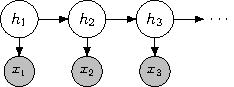
\includegraphics[width=0.45\columnwidth]{figures/hmm.pdf}
    \label{fig:examples-hmm}
  }
%  \subfigure[Directed grid model] {
%    \label{fig:examples-grid}
%    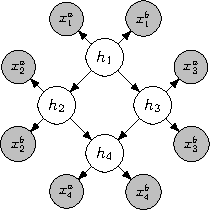
\includegraphics{figures/grid.pdf}
%  }
  \subfigure[Tree model] {
    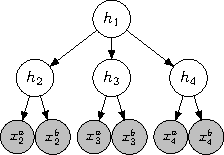
\includegraphics[width=0.45\columnwidth]{figures/tree.pdf}
    \label{fig:examples-tree}
  }
  \caption{Additional examples of models learnable using \LearnMarginals}
  \label{fig:examples}
\end{figure}

\paragraph{Hidden Markov Model}

In this example (\figureref{examples-hmm}), we assume that
  $\Pr(x_i|h_i) = O  ~\forall i$  and that $\Pr(h_{i+1} | h_i)
  = T ~\forall i$ (i.e. we have parameter sharing).
Note that while the first (and last) hidden variables $h_1, h_T$ in the
  sequence are not bottlenecks, they still have exclusive views ($x_1$ and
  $x_T$ respectively) whose parameters we know because they share
  parameters, $O$.
In step 1 of our algorithm, we use the bottleneck $h_2$ with views $x_1,
  x_2, x_3$ and solve $O$.
In step 2 of our algorithm, we can recover $\pi$ by solving for the
  unary clique $\{h_1\}$ and recover $T$ from the clique $\{h_{1},
  h_{2}\}$.

\paragraph{Latent Tree Structure}

In the latent tree structure (\figureref{examples-tree}), let the
  parameters be $\Pr(h_i) = \pi$, $\Pr(h_i | h_1) = T ~i \in \{2,3,4\}$
  and $\Pr(x^a_i | h_i) = \Pr(x^b_i | h_i) = O ~i \in \{2,3,4\}$.
Note that while $h_1$ is not directly connected to an observed variable,
  it is still a bottleneck, with views $x^a_2, x^a_3, x^a_4$.

In step 1, we recover the parameters $O$ from the bottleneck $h_2$ with
  views $\{x^a_2, x^b_2, x^a_3\}$. We also recover the conditional moments
  $\mOpp{2}{1}$, $\mOpp{3}{1}$, $\mOpp{4}{1}$ for $h_1$. 
In step 2, we can recover $\pi$ from the clique $\{h_1\}$, using any
  one of views (they are all exclusive). 
To recover $T$ from the clique $\{h_1, h_2\}$, we use the views $x^a_2$
  (exclusive to $h_2$) and $x^a_3$ (exclusive to $h_3$). Note that while
  $x^a_3$ is also a view for $h_2$, $x^a_3$ is independent of $h_2$ given
  $h_1$.

